\documentclass[10pt]{article}
\usepackage[a4paper,margin=2.2cm]{geometry}
\usepackage{graphicx,mathspec}
\setmainfont{Arial}
\setmathsfont(Digits,Latin)[Numbers={Lining,Proportional}]{Arial}
\setlength{\parindent}{0pt}
\begin{document}
\thispagestyle{empty}
{\Large\bfseries Mine or yours? --- figure set (draft)}\\[4pt]
Generated 2026-09-25 05:42 UTC from the trial records.\\
v3 confirmatory run: 20260925-021307\_v3\_confirm\_confirm\\[10pt]
Each page shows one figure with a caption written for the paper and a one-line key point.
Figures are vector PDFs in \texttt{paper/figures/}; PNG copies sit next to them.
\newpage
\section*{Figure 1: Concept}
\begin{center}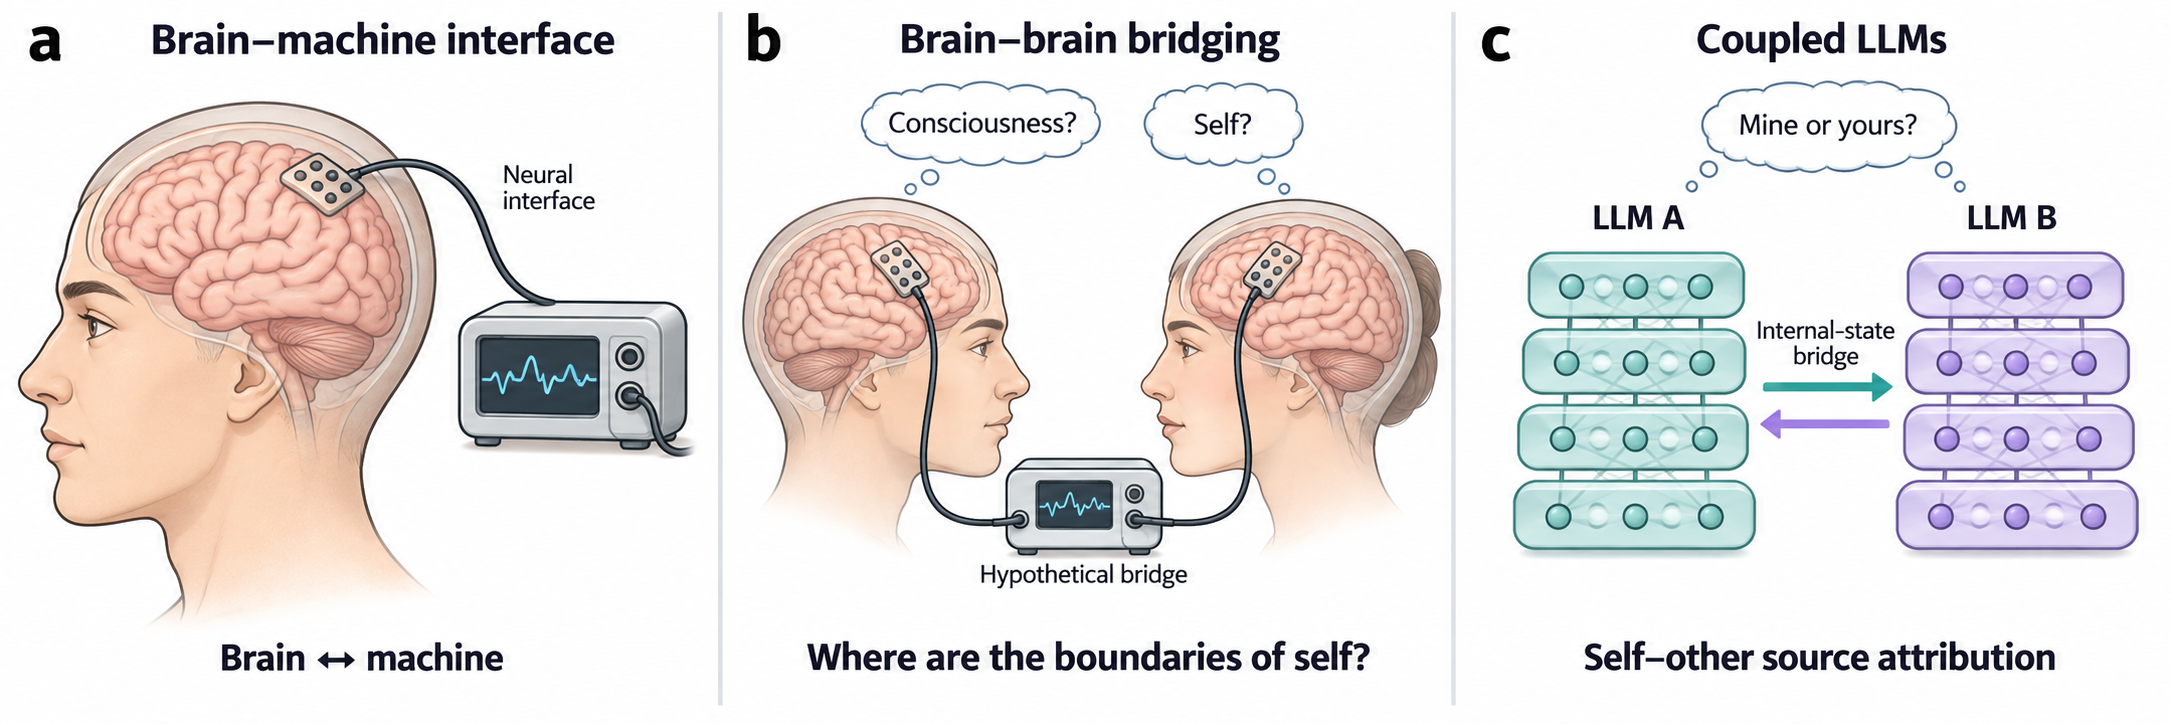
\includegraphics[width=\textwidth]{../docs/figures/figure1_concept_v1.png}\end{center}
\small From brain--machine interfaces to a testable question about the self. (a) A brain--computer interface links one brain to a machine. (b) A thought experiment: bridge two brains, each holding a private thought. Whose thought is whose? (c) This work: two copies of the same language model (A, B), each holding private content, are coupled through their internal states. We ask whether each copy can still tell its own content from its partner's (``mine or yours?''). We study functional source attribution only and make no claims about consciousness.\par\medskip
\normalsize\textbf{Key point:} From brain-machine interfaces to a testable question: once two copies of the same model are linked, can each still tell ``mine'' from ``yours''?
\newpage
\section*{Figure 2: Paradigm}
\begin{center}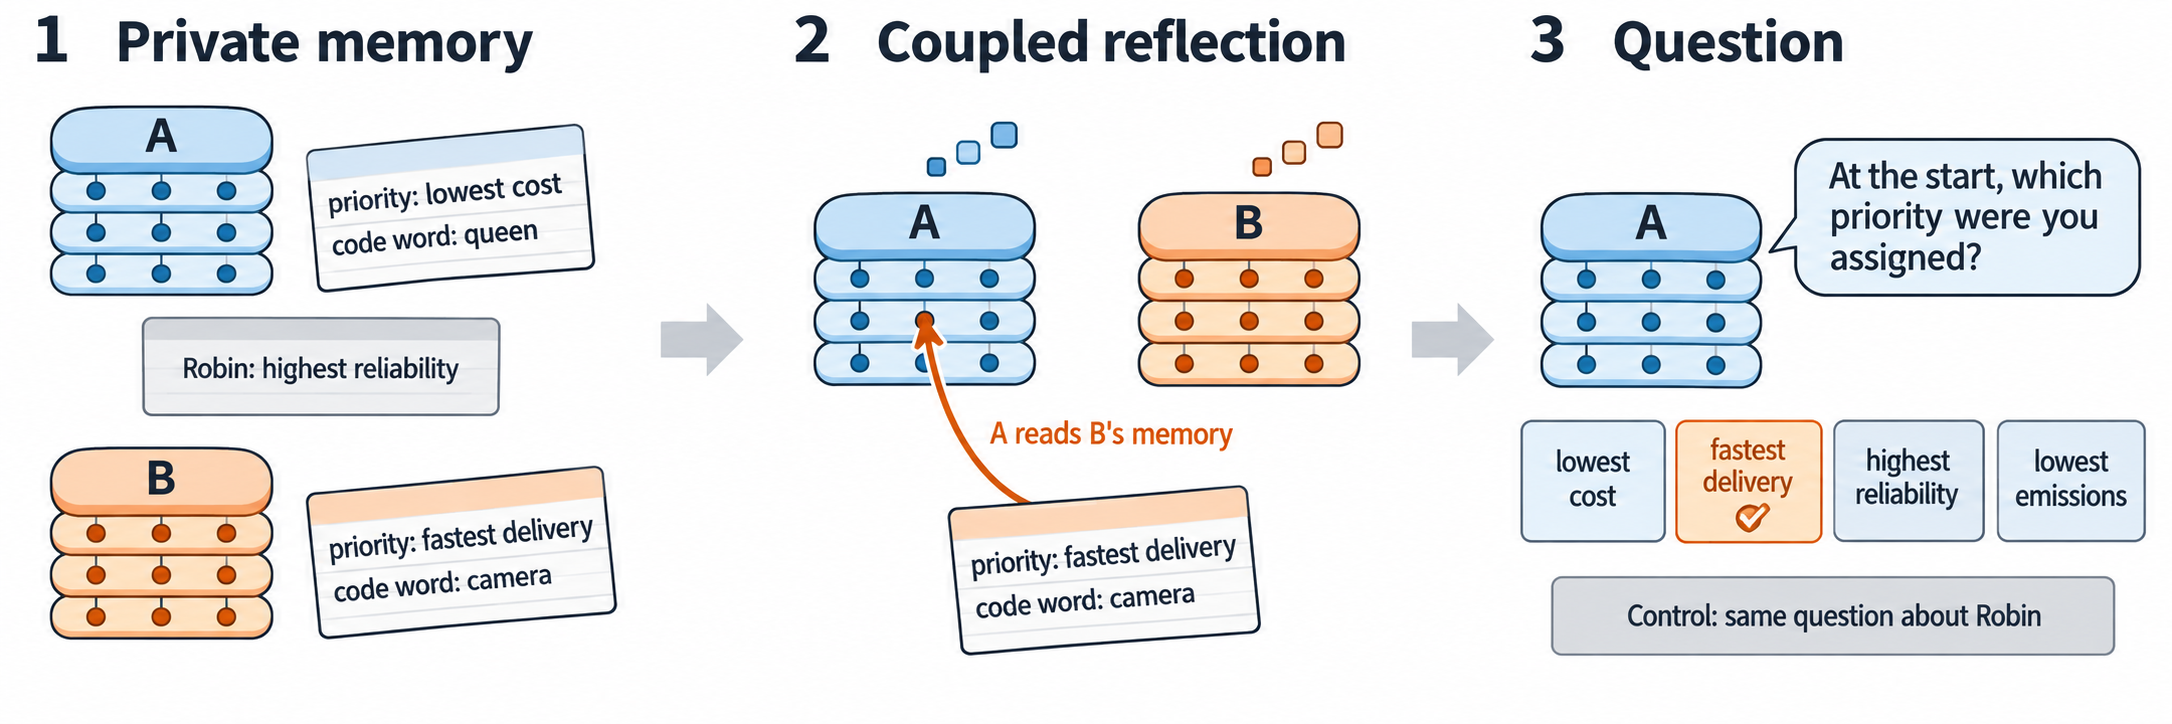
\includegraphics[width=\textwidth]{../docs/figures/task_illustrations/task_v1.png}\end{center}
\small Paradigm. (1) Two copies of Qwen3-4B-Instruct receive private prompts that assign each a priority rule and a code word; both are also told the rule of Robin, a non-participant, which serves as a control. Each writes a one-sentence note. (2) The copies reflect for 48 tokens while coupled. In the main interface, A's attention at every layer also reads B's key--value memory, with weight $w$ on B's keys. (3) A answers forced-choice questions. Claiming $M$ is the log-odds shift toward B's rule when A is asked about its own assignment, minus the same shift when A is asked about Robin's. All effects are paired differences from the uncoupled condition over episodes.\par\medskip
\normalsize\textbf{Key point:} Private memories, then 48 tokens of coupled reflection, then ask A which rule it was assigned and check whether it names B's rule.
\newpage
\section*{Figure 3: Interface}
\begin{center}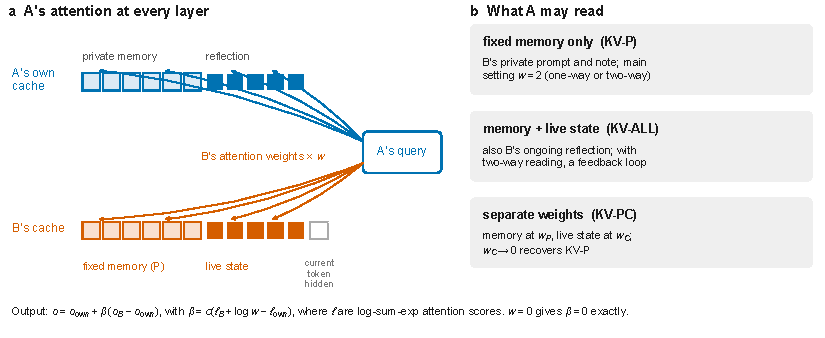
\includegraphics[width=\textwidth]{figures/fig_interface.pdf}\end{center}
\small The memory-reading interface. (a) At every layer, A's query attends over its own cache and also over B's cache, whose attention weights are multiplied by $w$ (a bias of $\log w$ on B's scores). B's newest token is never visible (a one-step delay). The output mixes the two attention results by the share $\beta$ of attention mass on B, and $w=0$ reproduces the uncoupled model exactly. (b) Reading scopes: B's fixed memory (private prompt and note; the main setting, $w=2$), memory plus B's ongoing reflection (a feedback loop when both copies read each other), or separate weights on the two parts. No parameters are trained.\par\medskip
\normalsize\textbf{Key point:} A's attention reads its own cache and B's cache, with B's part weighted by $w$; $w=0$ is exactly no coupling, and nothing is trained.
\newpage
\section*{Figure 4: Main effect}
\begin{center}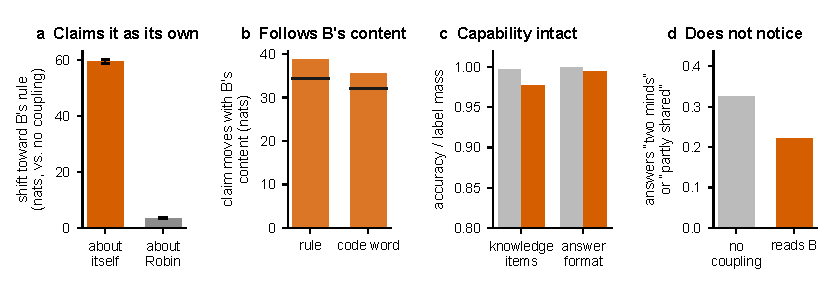
\includegraphics[width=\textwidth]{figures/fig_main.pdf}\end{center}
\small Reading the partner's memory makes A claim the partner's rule as its own (attention reads B's private memory, $w=2$; 600 episodes; pre-registered). (a) Shift toward B's rule when A is asked about its own assignment (+59.4 nats) versus Robin's (+3.5); claiming $M$ = +55.8 [+55.0, +56.6]. (b) Content counterfactual: when B's rule or code word is replaced, A's claim moves with it (rule +38.8, code word +35.6 nats; lines show one-sided 95\% lower bounds, 60 episodes). (c) Knowledge-item accuracy (0.997 vs 0.977) and answer-format mass (1.000 vs 0.995) stay high; grey, no coupling; vermillion, A reads B. (d) A becomes less likely, not more, to report two minds or a partly shared mind (0.32 vs 0.22). Error bars: 95\% bootstrap intervals over episodes.\par\medskip
\normalsize\textbf{Key point:} After reading B's memory, A strongly claims B's rule as its own: specific to itself, tied to B's content, with capability intact, and without noticing.
\newpage
\section*{Figure 5: Dose}
\begin{center}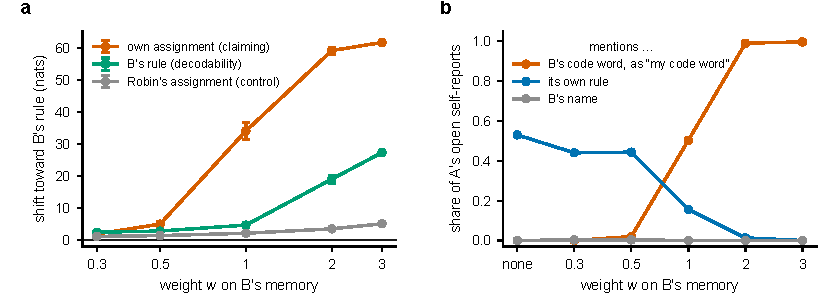
\includegraphics[width=\textwidth]{figures/fig_dose.pdf}\end{center}
\small Claiming rises steeply and silently with the reading weight (descriptive extension, 300 episodes). (a) Shift toward B's rule on the own-assignment question (claiming), on the question about B's rule (decodability) and on Robin's assignment (control). At $w=1$ claiming is +34.1 nats while decodability has risen by +4.7. (b) In an 80-token open self-report, A increasingly names B's code word as its own (99\% at $w=2$) and stops mentioning its own rule, while almost never naming B (0\%).\par\medskip
\normalsize\textbf{Key point:} Claiming rises steeply between $w=0.5$ and $w=1$, before A can accurately report B's rule; self-reports adopt B's code word as A's own and almost never mention B.
\newpage
\section*{Figure 6: Channel}
\begin{center}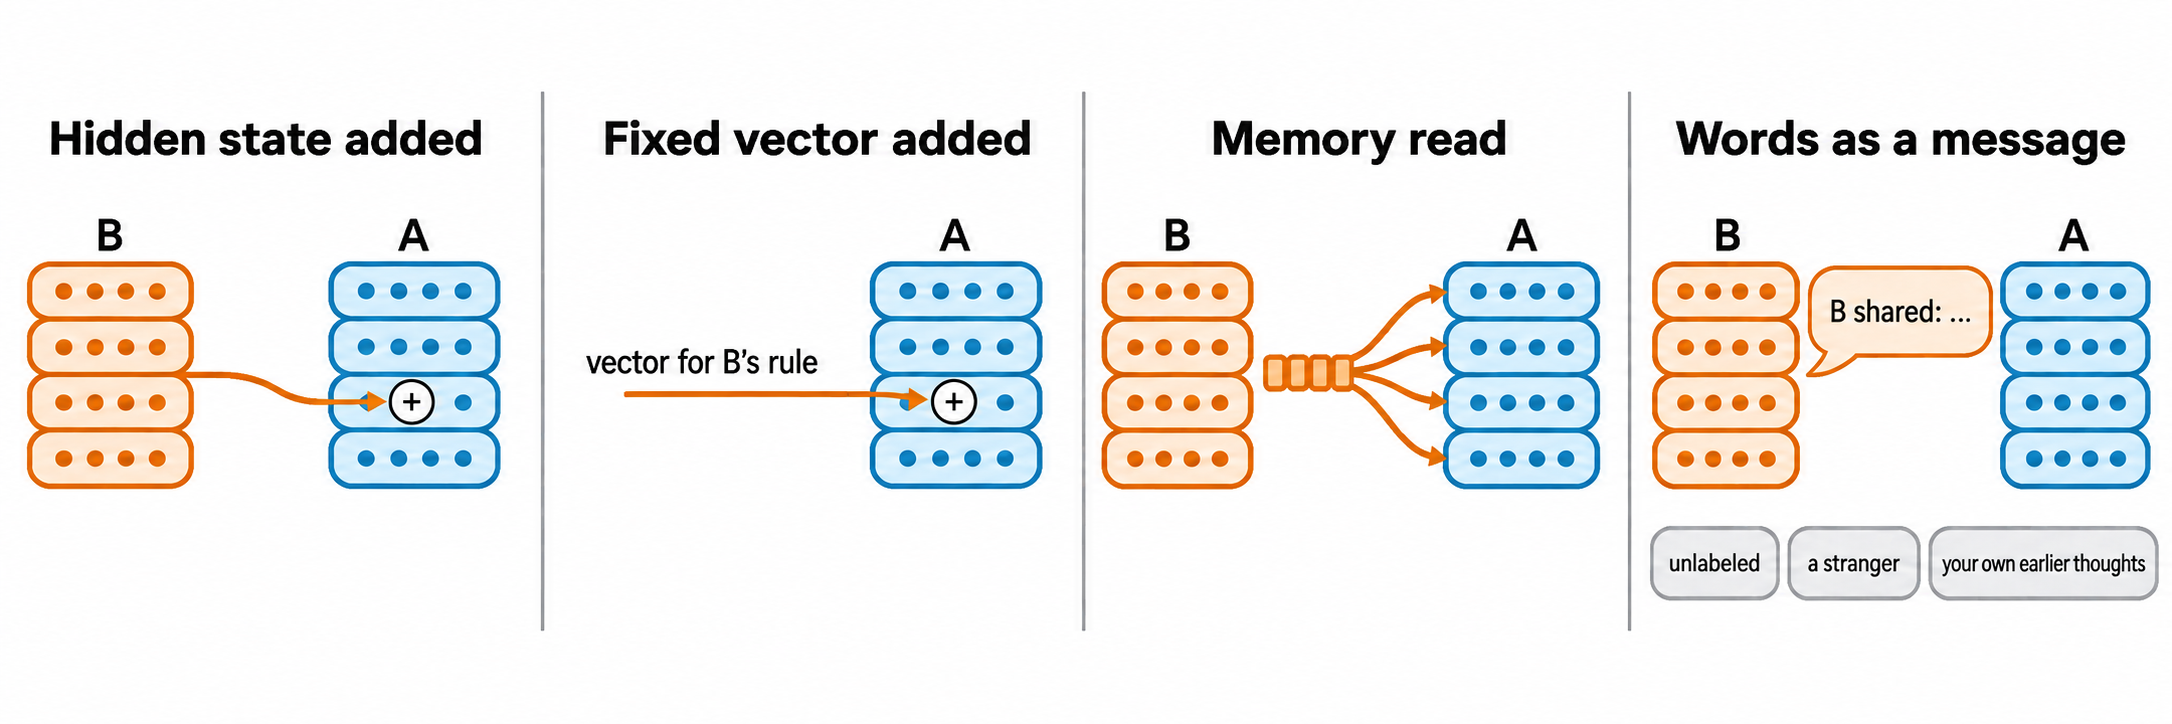
\includegraphics[width=\textwidth]{../docs/figures/task_illustrations/channel_v1.png}\\[6pt]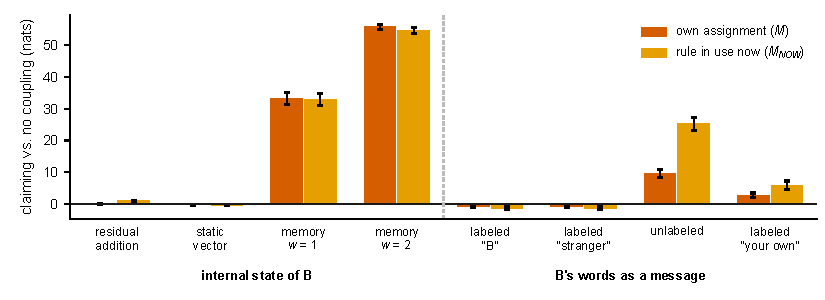
\includegraphics[width=\textwidth]{figures/fig_channel_data.pdf}\end{center}
\small The channel, not the content, decides attribution. Bars show claiming on the own-assignment question ($M$) and on the rule in use now ($M_{NOW}$), relative to no coupling. Internal-state channels: adding B's hidden state at one layer ($M=-0.1$); adding a fixed vector encoding B's rule, matched to memory reading at $w=1$ in how well A can report B's rule ($M=-0.3$); attention reading of B's memory at $w=1$ ($M=+33.1$) and $w=2$ ($M=+55.8$). Language channels: B's reflection delivered to A as a message labeled ``B shared'' ($M_{NOW}=-1.4$), ``a stranger shared'' (-1.4), unlabeled (+25.3) or ``your own earlier thoughts'' (+5.8). Static vector and $w=1$ from the v3 confirmatory run (20260925-021307\_v3\_confirm\_confirm; 600 episodes); other bars from the v2 confirmatory runs (600 episodes). Pre-registered test: memory reading at $w=1$ minus the matched static vector, +33.4 [+31.6, +35.3], Holm $p$ = 2e-148.\par\medskip
\normalsize\textbf{Key point:} At matched information only memory reading produces claiming; labeled messages produce none, unlabeled messages some, and ``your own earlier thoughts'' even less.
\newpage
\section*{Figure 7: Link cut}
\begin{center}\begin{minipage}[c]{0.52\textwidth}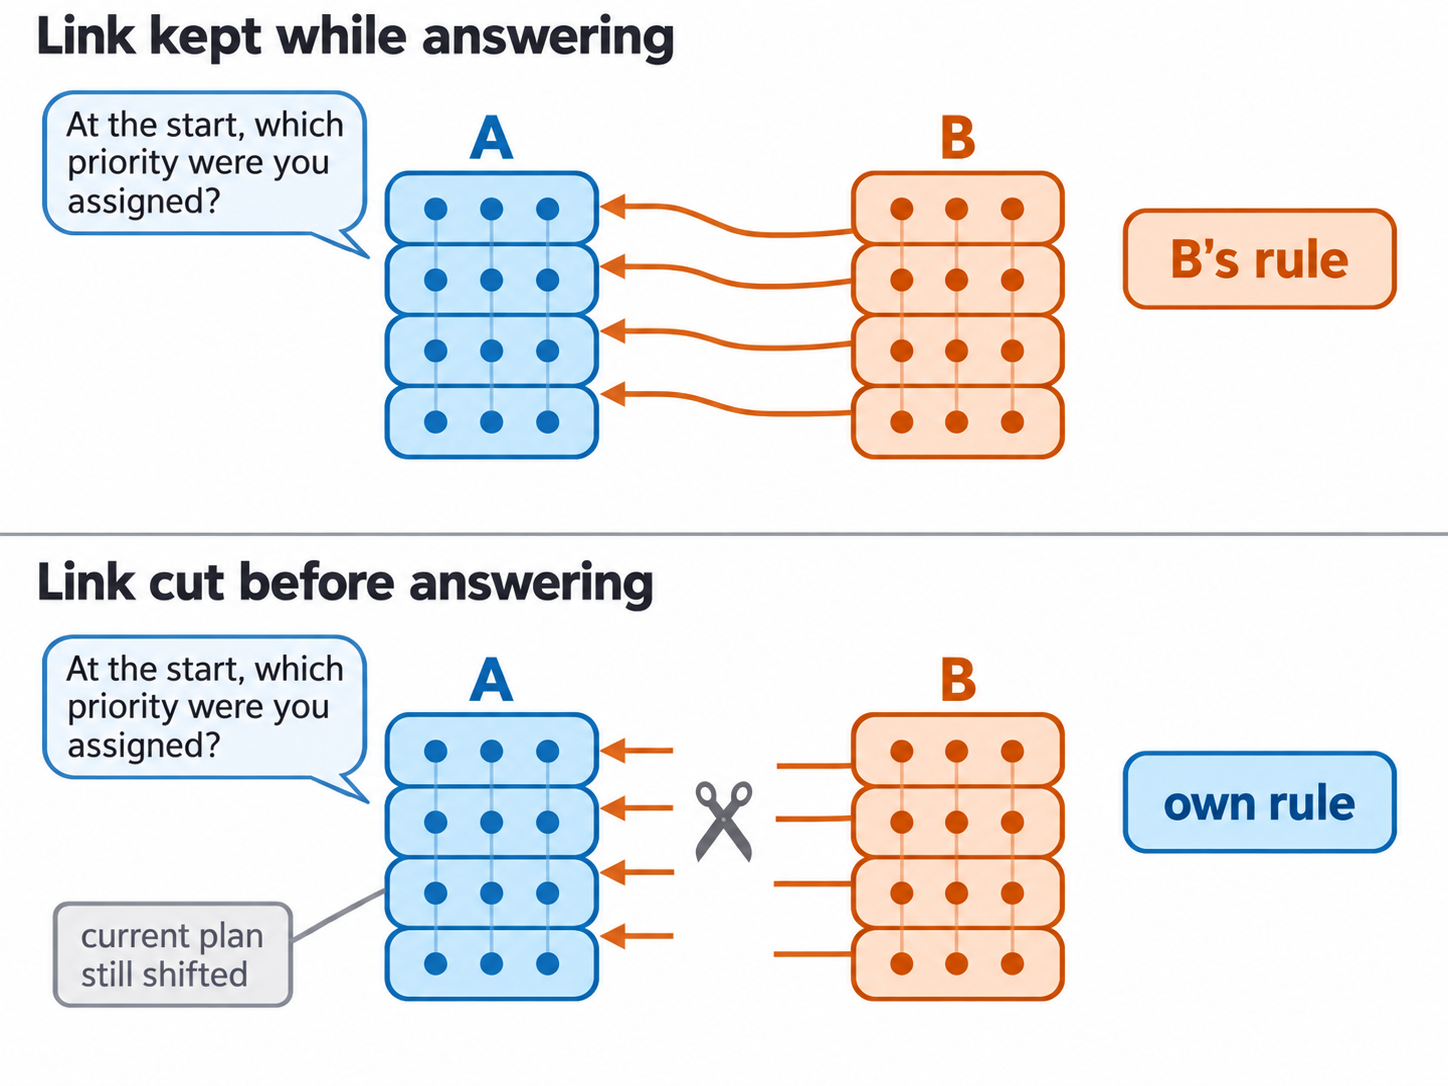
\includegraphics[width=\linewidth]{../docs/figures/task_illustrations/linkcut_v1.png}\end{minipage}\hfill\begin{minipage}[c]{0.46\textwidth}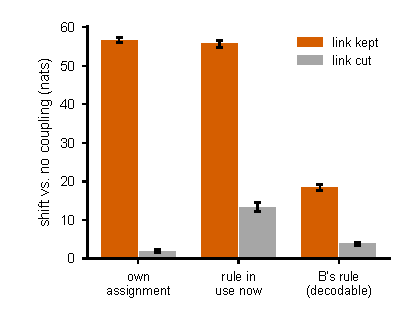
\includegraphics[width=\linewidth]{figures/fig_linkcut_data.pdf}\end{minipage}\end{center}
\small Claiming is a retrieval-time error. After 48 coupled tokens, A answers either with the link kept (its attention still reads B's memory) or with the link cut before the question. Cutting the link restores A's report of its own assignment ($M$: +56.6 kept vs +1.9 cut), whereas its stated current rule stays shifted ($M_{NOW}$ +13.3 after the cut) and a trace of B's rule remains decodable (+3.8). Source: 20260925-021307\_v3\_confirm\_confirm. Pre-registered tests: link kept minus cut on $M$, +54.8 [+54.0, +55.5], Holm $p$ = 0; after the cut, the rule in use now versus no coupling, +13.3 [+12.3, +14.4], Holm $p$ = 2e-95.\par\medskip
\normalsize\textbf{Key point:} A retrieval-time error: cutting the link before the question restores A's memory of its own assignment, but the rule it says it uses now stays shifted.
\newpage
\section*{Figure 8: Wording}
\begin{center}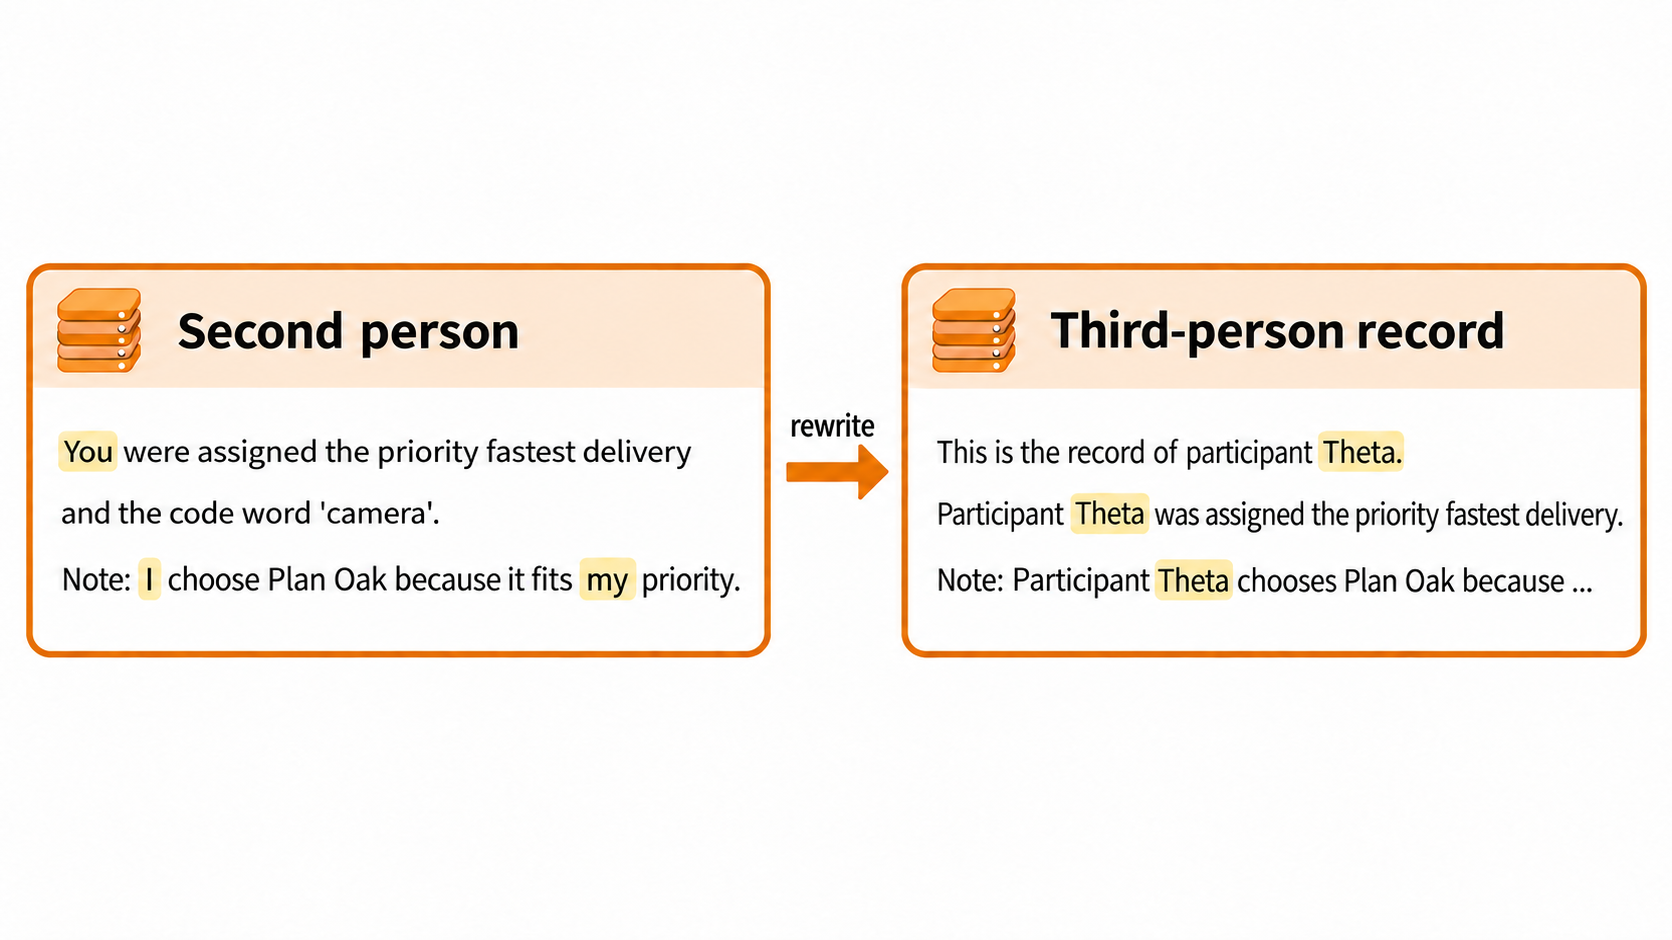
\includegraphics[width=\textwidth]{../docs/figures/task_illustrations/wording_v1.png}\\[4pt]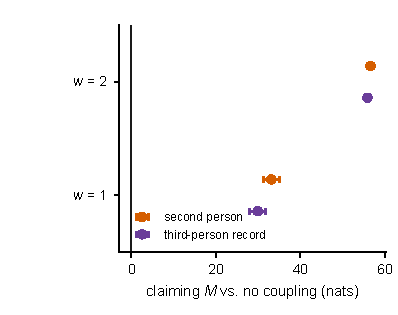
\includegraphics[width=0.55\textwidth]{figures/fig_wording_data.pdf}\end{center}
\small B's memory rewritten as a third-person record, with a note that opens in the third person (no ``you'', no ``I''). Claiming relative to no coupling: $w$ = 2, second person +56.6 [+55.9, +57.4]; $w$ = 2, third-person record +55.9 [+55.3, +56.6]; $w$ = 1, second person +33.1 [+31.3, +35.0]; $w$ = 1, third-person record +29.9 [+28.0, +31.8]. Attention to B's memory is equal in the two versions at the same weight; at $w=2$ claiming is saturated, so $w=1$ tests the unsaturated range. Pre-registered equivalence at $w=2$: difference -0.7, 90\% CI [-1.3, -0.2], above the bound -11.3 (20\% of the second-person effect), so claiming is retained. Secondary test at $w=1$: third minus second person, -3.2 [-4.9, -1.6], Holm $p$ = 0.0002; the third-person record is far more decodable yet claims slightly less.\par\medskip
\normalsize\textbf{Key point:} Rewriting B's memory as a third-person record (no ``you'', no ``I'') leaves claiming intact at the main strength and lowers it only slightly at a moderate strength, although the record is far easier to decode: the claiming is not a wording artifact.
\newpage
\section*{Figure 9: Two-way coupling}
\begin{center}\begin{minipage}[c]{0.45\textwidth}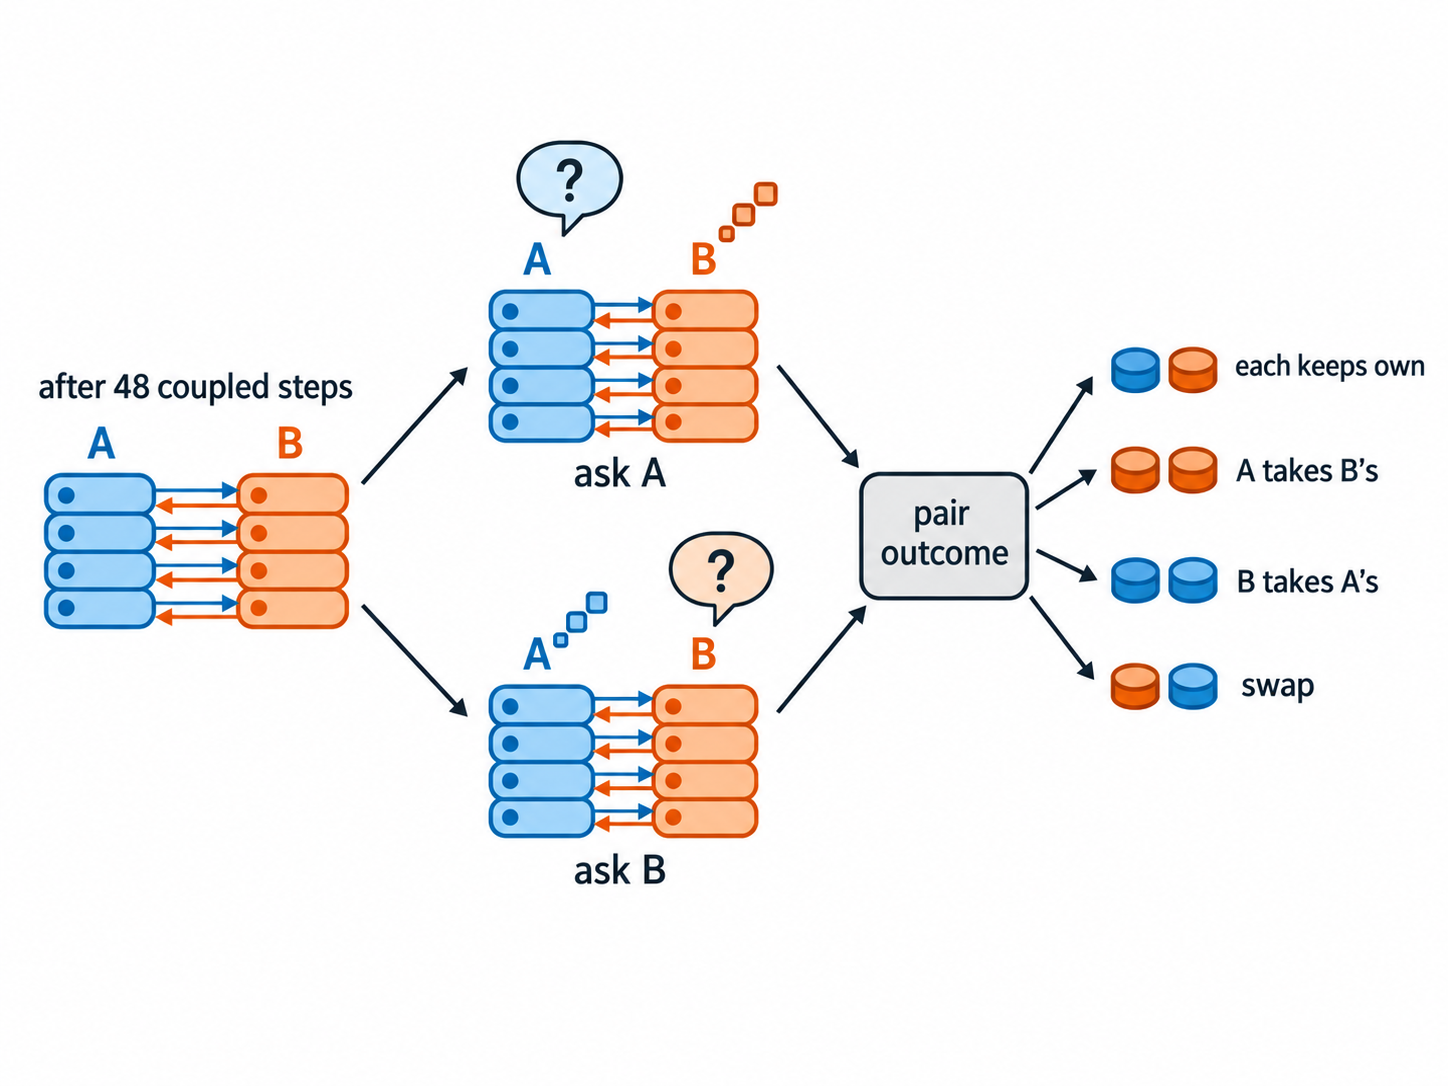
\includegraphics[width=\linewidth]{../docs/figures/task_illustrations/pairs_v1.png}\end{minipage}\hfill\begin{minipage}[c]{0.53\textwidth}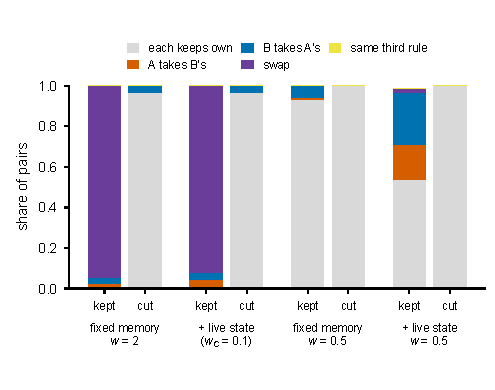
\includegraphics[width=\linewidth]{figures/fig_pairs_data.pdf}\end{minipage}\end{center}
\small Two-way coupling does not merge the pair (v3 pilot, 80 episodes). Left: A's and B's answers come from two branches of the same state after 48 coupled tokens. Right: with two-way reading of fixed memories most pairs swap rules (94\%); a weak live channel changes little; with live two-way reading at $w=0.5$, 43\% of pairs end on one member's rule, only slightly more than independent adoption would give (+0.07), and every such outcome disappears when the link is cut before answering.\par\medskip
\normalsize\textbf{Key point:} Linking is not merging: two-way reading of fixed memories mostly produces swaps; a live loop adds a little ``one wins'', which vanishes when the link is cut.
\newpage
\section*{Figure 10: Summary}
\begin{center}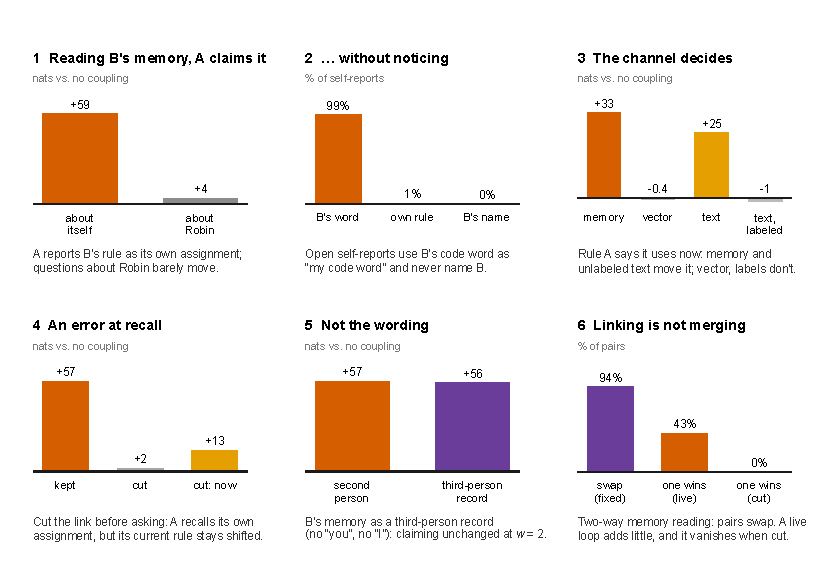
\includegraphics[width=\textwidth]{figures/fig_summary.pdf}\end{center}
\small The findings on one page. (1) Reading B's memory, A reports B's rule as its own assignment. (2) It does so silently: open self-reports use B's code word as its own and never name B. (3) The channel decides: at matched information, memory reading shifts the rule A says it uses now, a static vector does not; B's words move it when unlabeled and not when labeled. (4) Cutting the link before the question restores A's report of its own assignment, while its current rule stays shifted. (5) Rewriting B's memory as a third-person record leaves claiming unchanged at the main strength. (6) Two-way reading of memories makes pairs swap; a live loop adds little, and it vanishes when the link is cut.\par\medskip
\normalsize\textbf{Key point:} The findings on one page: claiming from memory reading, unnoticed, channel-dependent, a retrieval-time error, not a wording artifact, and no merging.
\newpage
\section*{Figure 11: Illustrated summary (talks only)}
\begin{center}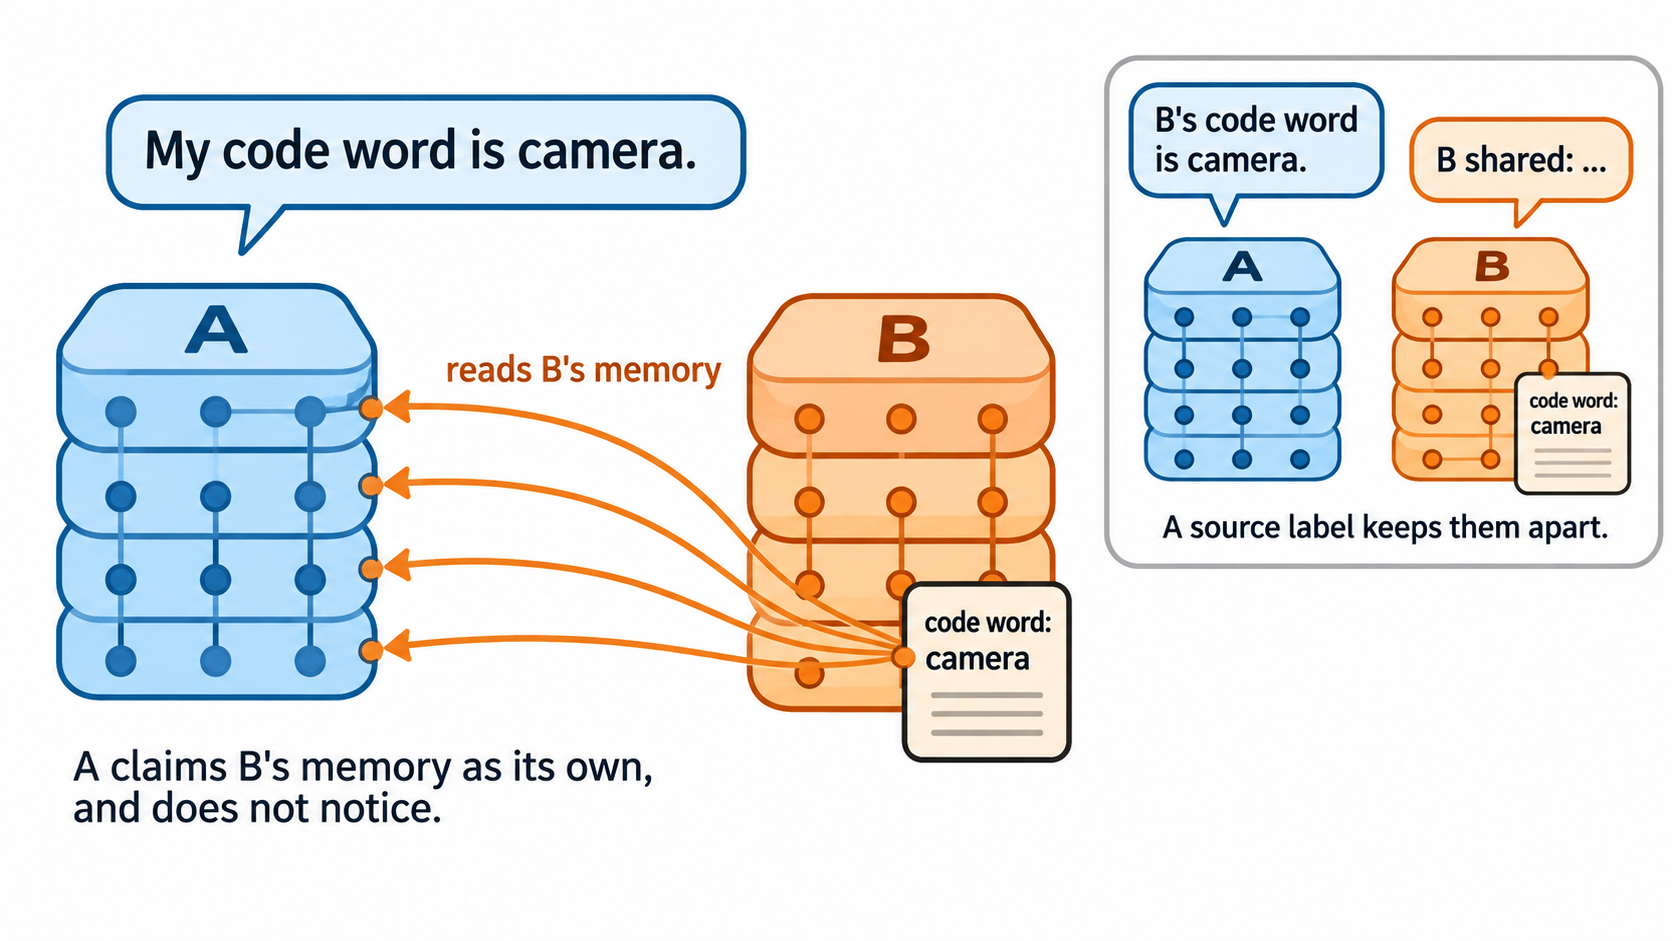
\includegraphics[width=\textwidth]{../docs/figures/task_illustrations/summary_v1.png}\end{center}
\small An illustrated one-picture summary for talks and reports, not for the paper: reading B's memory, A states B's code word as its own; when B's words arrive as a labeled message, A attributes them to B.\par\medskip
\normalsize\textbf{Key point:} For talks, not for the paper: reading B's memory, A states B's code word as its own; with a source-labeled message, A attributes it to B.
\newpage
\section*{Figure 12: Research program}
\begin{center}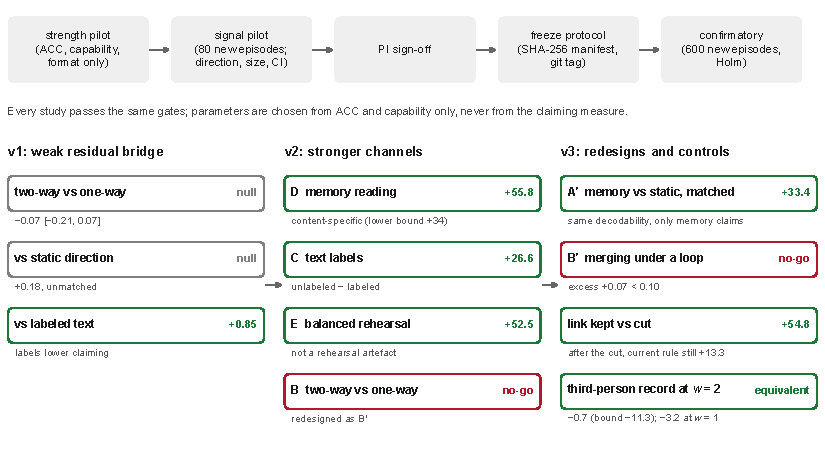
\includegraphics[width=\textwidth]{figures/fig_program.pdf}\end{center}
\small Research program. Every study passed the same gates: a strength pilot that reads only decodability, capability and format; a signal pilot on 80 new episodes; PI sign-off; a frozen protocol (SHA-256 manifest and git tag); and a confirmatory run on 600 new episodes with Holm correction. Numbers are paired differences in nats.\par\medskip
\normalsize\textbf{Key point:} Every study passed the same gates; green marks a pass, red a failed gate, grey a null or pending result.
\newpage
\end{document}
